% Network findings. Story: (1) cuisines differ mostly in WHAT they use;
% (2) a distinctive pair is not always combined on purpose; (3) so we score
% WHAT and HOW separately for every recipe.
% The longer recipe-projection analyses live in docs/ (not in the paper).

\subsection*{Cuisines differ mostly in which ingredients they use}
We built a bipartite network with 26,727 recipes, 3,877 ingredients, and 227,965 links, where a link means that the ingredient appears in the recipe. Two ingredients are then joined when they appear in the same recipe (271,443 pairs). Fig.~\ref{fig:network} shows the strongest of these links for the most distinctive ingredients of each cuisine. Ingredients of the same cuisine end up together: 21\% of the links shown join two ingredients of the same cuisine, against 10\% when the colors are shuffled. Chinese, Japanese and Thai ingredients sit close to each other around soy sauce, and Italian, Greek and French ones around olive oil.

The cuisine tags are written by Food.com users, so we checked that they agree with the ingredients. We linked every recipe to the recipes with the most similar ingredient lists, without looking at the tags. In this recipe network, 63.0\% of the link weight joins two recipes with the same tag. With shuffled tags it is 17.1\%.

Is this because cuisines use different ingredients, or because they combine them differently? We shuffled ingredients among the recipes of each cuisine, so that every recipe kept its number of ingredients and every ingredient stayed as common in the cuisine as before, but the combinations became random. The within-cuisine share was still 59.3\%, below the real 63.0\% in all 49 shuffles. For whole cuisines, then, almost all of the difference is in \emph{what} they use, and \emph{how} adds a few points. The following sections ask the same question for single recipes.

\begin{figure}[tbhp]
\centering
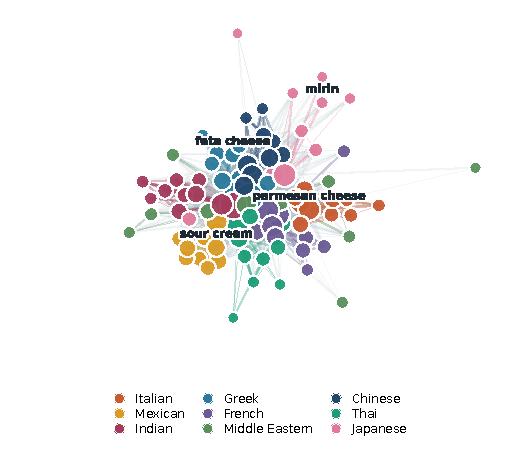
\includegraphics[width=8.7cm]{figures/ingredient_backbone.pdf}
\caption{The ingredient network, reduced to its strongest links. Each node is an ingredient: the ten most distinctive of each cuisine and a few very common ones, sized by its number of recipes and colored by the cuisine where it is most distinctive. Two ingredients are linked when they share at least 30 recipes and the link passes the disparity filter \cite{serrano2009extracting} ($\alpha < 0.005$), which keeps a link only if it carries a larger share of an ingredient's co-occurrences than it would if they were spread evenly over its neighbors. Positions come from the links alone. Ingredients of the same cuisine end up together: 21\% of the links join two nodes of the same color, against 10\% (at most 12\%) in 2,000 shuffles of the colors.}
\label{fig:network}
\end{figure}

\subsection*{A distinctive pair is not always combined on purpose}
Following Ahn et al. \cite{ahn2011flavor}, we measured how much more often each ingredient pair appears in one cuisine than, on average, in the other eight. Green onion and soy sauce appear together in 24.1\% of Chinese recipes, against 2.9\% on average elsewhere. Feta cheese and olive oil are 20.9 percentage points more common in Greek recipes, and fish sauce and lime juice 16.0 points more common in Thai recipes.

A pair can be distinctive simply because both ingredients are common in the cuisine. To separate \emph{what} from \emph{how}, we took the most distinctive pair of each cuisine as nine examples and compared each with 49 randomized networks (Fig.~\ref{fig:pairs}A). In these networks every recipe keeps its number of ingredients and every ingredient stays as common as before within its cuisine and dish type; only the combinations change. Seven of the nine pairs appeared together more often than the central 95\% of these networks. Mexican recipes combined chili powder and cumin 697 times, almost twice the randomized median of 353: the two are combined on purpose. Italian recipes combined olive oil and parmesan cheese 1,277 times, which is fewer than the randomized median of 1,437: the pair is distinctive of Italian recipes only because each of the two ingredients is common there.

\begin{figure*}[t!]
\centering
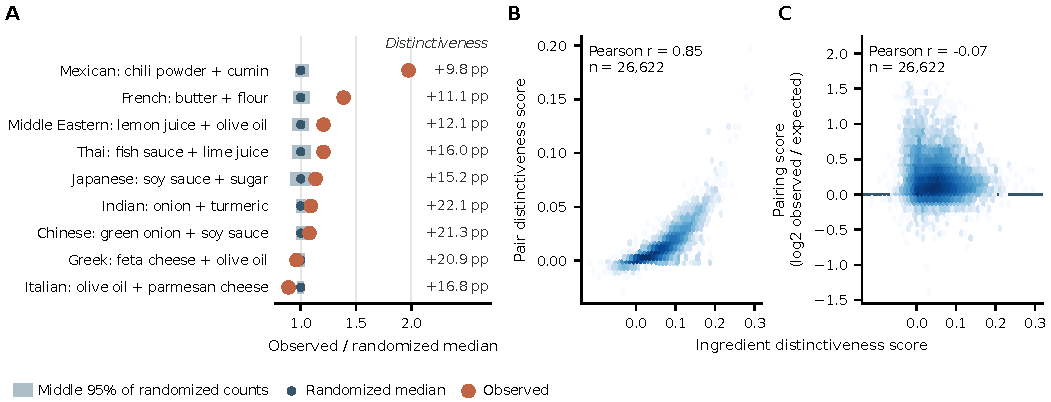
\includegraphics[width=17.8cm]{figures/pairs_and_scores.pdf}
\caption{What a recipe uses and how it combines it are different measurements. (A) For the most distinctive pair of each cuisine, the number of recipes containing both ingredients divided by the median over 49 randomized networks that keep each recipe's number of ingredients and each ingredient's frequency within its cuisine and dish type. The gray interval is the middle 95\% of the randomized counts; the number next to each pair is its distinctiveness in percentage points. Points to the right of the interval are pairs combined more often than their popularity predicts. (B) Ingredient score against pair score for every recipe; darker hexagons contain more recipes. The two are nearly the same measurement. (C) Ingredient score against pairing score: knowing what a recipe uses says almost nothing about how unusually it combines it.}
\label{fig:pairs}
\end{figure*}

\subsection*{What and how are two different scores}
We turned these measures into three scores per recipe. The \emph{ingredient score} is the mean distinctiveness of the recipe's ingredients (\emph{what}). The \emph{pair score} is the mean distinctiveness of its ingredient pairs. The \emph{pairing score} (\emph{how}) repeats the comparison of Fig.~\ref{fig:pairs}A for every pair of the recipe: the number of recipes of the cuisine that contain both ingredients, divided by the number expected in the randomized networks. A pair found twice as often as expected counts $+1$, a pair found as often as expected counts 0, and a pair found half as often counts $-1$ (the $\log_2$ of the ratio), and the score is the mean over the recipe's pairs (Methods). We could score 26,622 of the 26,727 recipes; 105 had fewer than two retained ingredients.

The ingredient and pair scores are strongly correlated ($r=0.85$; Fig.~\ref{fig:pairs}B): a recipe with distinctive pairs is almost always a recipe with distinctive ingredients, so the pair score adds little. The pairing score is different. Its correlation with the ingredient score is $r=-0.07$ (Fig.~\ref{fig:pairs}C) and with the pair score $r=0.06$, so knowing which ingredients a recipe uses says almost nothing about whether it combines them in the usual way. Its highest-scoring pairs are recipe templates: carrot and celery in Italian recipes (the base of a soffritto; 184 recipes against 19 expected), garlic and ginger paste in Indian recipes (76 against 4.0), tequila and triple sec in Mexican recipes (45 against 1.4), and bay leaf and thyme in French recipes (39 against 7.1). Not all templates are traditional: garlic powder with onion powder, or the canned cream soups of Mexican casseroles, also score high.
